\documentclass[12pt]{article}
\usepackage[a4paper,portrait,margin=0.5in]{geometry}

\usepackage{amsmath}
\usepackage{amssymb}
\usepackage{amsthm}
\usepackage[toc,page]{appendix}
\usepackage{graphicx}
\usepackage{caption}
\usepackage{placeins}
\usepackage{float}
\usepackage{tabularx}
\usepackage{array,booktabs}
\usepackage{bm}
\usepackage{bbm}
\usepackage{siunitx}
\usepackage[skip=0pt]{caption}
\newcommand{\czt}{\tilde{c}_2}
\newcommand{\cdt}{\tilde{c}_3}
\newcommand{\DKL}{D_\mrm{KL}}
\newcommand{\Eden}{E^\mrm d}
\newcommand{\Esom}{E^\mrm s}
\newcommand{\ipsum}{{\bf IPSUM}}
\newcommand{\lb}{\left}
\newcommand{\lorem}{{\bf LOREM}}
\newcommand{\mb}{\mathbf}
\newcommand{\mrm}{\mathrm}
\newcommand{\mV}{\milli\volt}
\newcommand{\N}{\mathbb N}
\newcommand{\R}{\mathbb R}
\newcommand{\rb}{\right}
\newcommand{\Spre}{\Sigma_{\mrm{usp}}}
\newcommand{\todoin}[1]{\todo[inline]{#1}}
\newcommand{\todosolved}[1]{\todo[inline, color=green]{#1}}
\newcommand{\un}{\mb{1}}
\newcommand{\wden}{w^\mrm d}
\newcommand{\wsom}{w^\mrm s}
\newcommand{\xeps}{\mathbf x^{\epsilon}}

\begin{document}
\setlength{\abovedisplayskip}{3pt}
\setlength{\belowdisplayskip}{3pt}
{\center\bf Abstract}\\
Due to their simplicity and success in machine learning, gradient based learning rules represent a popular choice for synaptic plasticity models. While they have been linked to biological phenoma such as STDP, it is often ignored that their predictions generally depend on a specific representation of the synaptic strength. Unlike in an artifical neural network, where the weight of a synaptic input is just an abstract variable, in a neuron, the impact of a synapse corresponds simultaneously to the state of many physical quantities inside the cell. Which one we choose to derive a gradient descent learning rule can have a remarkable effect in terms of model prediction.
This is dissatisfying both from the viewpoint of optimal output adaptation, as well as from a conceptual angle. Clearly, the aim of learning is to adapt the output statistics rather than an internal parameter, and plasticity should strive to adjust it in an optimal fashion. From an evolutionary perspective the contribution of local synaptic changes to the change in output should be independent of parameters such as the synapse's random location on the dendritic tree. 
Natural gradient descent provides a solution to both problems by following the gradient on the manifold of the neuron's firing distributions, combining the intuition of gradient descent with the elegance of an output change that is invariant under a change of representation. While the computational advantages of natural gradient are well-studied, its predictive power as a model for in-vivo synaptic plasticity has not been assesed. We study it from a biological perspective by applying it to learning with spiking neurons,  and demonstrate that it exhibits faster convergence compared to classical gradient learning. Furthermore, natural gradient predicts plasticity phenomena such as learning rate scaling in distal dendrites and provides a unified framework for both homo- and heterosynaptic plasticity.
{\center\bf Additional Detail}\\
We explore the biological predictions of natural gradient descent learning (Amari 1998, Ollivier 2015), by calculating an explicit formula for the synaptic weight update in the context of a supervised learning task with Poisson spiking neurons (see Fig 1A). In terms of somatic EPSP amplitudes the weight update is then given as 
\begin{eqnarray}
\label{Results_Natural_Gradient}
\dot{\mb w} =\eta \ \gamma_{\mrm s} \lb(Y^*-\phi(V)\rb) \frac{\phi'(V)}{\phi(V)}\lb(\frac{c_{\epsilon}\xeps}{\mb r}-\gamma_{\mrm u}+\gamma_{\mrm w}{\mb w}\rb),
\end{eqnarray} 
where $Y^*$ denotes the teacher spiking, and the firing of the student neuron depends via a nonlinearity $\phi$ on the somatic membrane potential $V$. The latter is given as the sum $V=\sum_i w_i x_i^{\epsilon}$ of the unweighted synaptic potentials $x_i^{\epsilon}$ (USP), evoked by presynaptic input, weighted by the somatic amplitudes $w_i$. While the coefficients $\gamma_{\mrm s},\gamma_{\mrm u},\gamma_{\mrm w}$ are in general functions of the membrane potential, its first and second moment, as well as the total input, our simulations indicate that in many cases, $\gamma_{\mrm u},\gamma_{\mrm w}$ may be replaced by constants, while $\gamma_{\mrm s}$ yields a global scaling dependent on the properties of the spiking-nonlinearity.
A closer look at Equation \ref{Results_Natural_Gradient} reveals, that just as classical gradient descent based learning rules, natural gradient plasticity follows the postsynaptic error. Additionally, a presynaptic contribution adjusts synapses that received input close to the current point in time. However, unlike for classical gradient learning, this homosynaptic weight update is complemented by both a uniform as as well as a weight proportional heterosynaptic contribution. This is in line with experimental findings that show that also currently unstimulated synapses undergo plasticity if their neighbours receive input (Lynch 1977, Chistiakova 2009), as well as with computational studies that list heterosynaptic plasticity as a necessary component of stable learning (Zenke 2017). Qualitatively similar to experimental findings in different parts of the brain (Lynch 1970 White 1990, Royer \& Paré 2003 Wöhrl 2007), we found that given a simple stimulation protocol, changes at unstimulated synapses exhibited an opposite sign compared to the plasticity at stimulated synapses, thereby keeping the synapse within their operational range.
Additionally, our learning rule also includes a synapse-specific scaling of the homosynaptic contribution by the input rate, similar to the rescaling observed in the Bayesian plasticity framework (Aitchison 2014?). The rescaling arises from a normalization by the USP variance, and simulations revealed that under a simple stimulation protocol, the learning rate of the full natural gradient rule was inversely related to the USP variance when the mean of the USP was kept fixed. 
We also derived a version of our learning rule in terms synaptic EPSP amplitudes. Since synaptic changes are attenuated on their way to the soma, in order to evoke the same effect in terms of adapting the neuron's firing behavior, changes at distal synapses must be increased compared to plasticity at proximal synapses with a similar impact on output firing. This phenomenon of democratic plasticity reminds of the dendritic democracy concept (Häusser 2001, Magee and Cook 2000), but can exist independent from the latter.
Our results demonstrate that apart from a consistent plasticity framework that is optimal in terms of output adaptation, natural gradient descent learning provides several experimentally testable predictions, and in particular a unified framework for both homo-and heterosynaptic changes.
\begin{figure}
\center
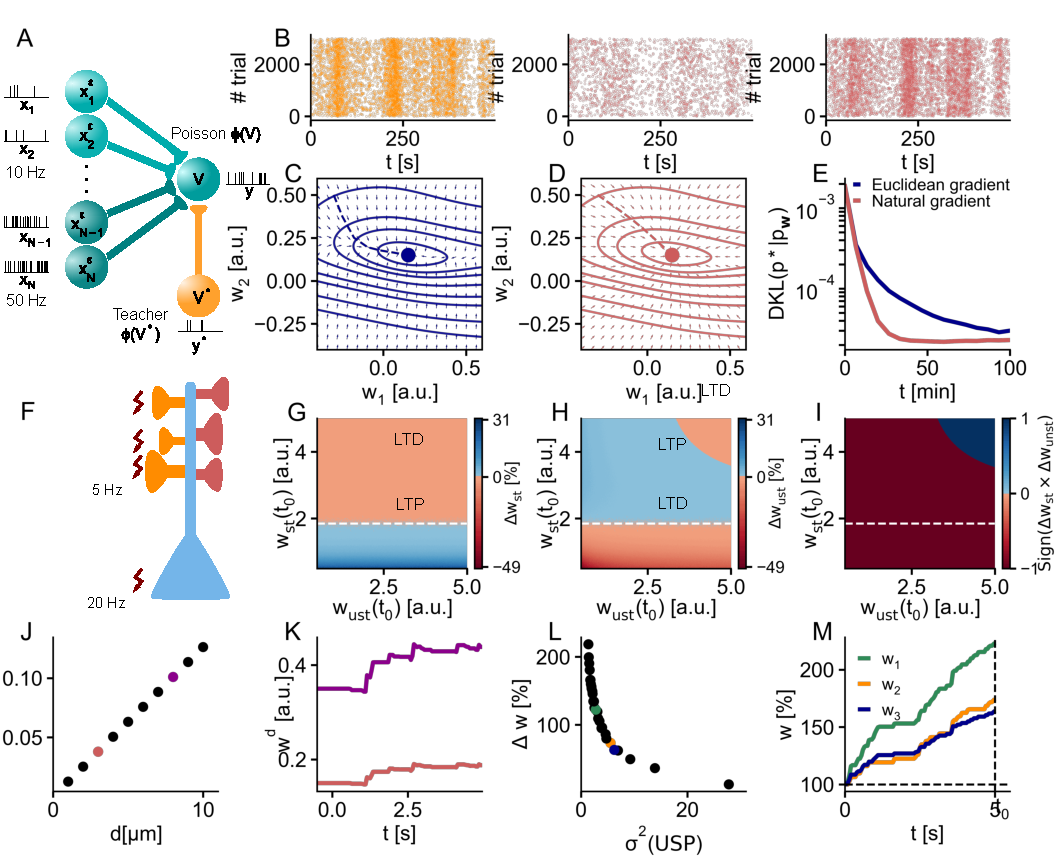
\includegraphics[scale=1.0]{Figure_Cosyne2}
\vspace{-0.7cm}
\caption{\footnotesize{\bf A} Learning task. Receiving Poisson spike trains from afferent nerve cells, a neuron had to respond by firing spikes according to a target distribution. The latter was delivered via spikes from a teacher neuron that received the same input. The firing rate of the student neuron depended via a transfer function $\phi$ on the somatic membrane potential $V$, whose elevation above rest was determined by the sum of the synaptic inputs.{\bf(B-D)} Spike trains, for teacher (orange) and student (red) neuron. ({\bf(B)} before learning, {\bf (C)} after learning with the natural gradient rule).{\bf{(E-G)}} Contour lines of the $\DKL$ between output and target distribution and normalized vector plots for Euclidean gradient vectors{\bf(E)} and natural gradient vectors {\bf(F)} together with weight path during learning. The classical error learning rule based on Euclidean gradient descent follows the contour lines of the error function, whereas the natural gradient rule updates synapses in direction of the target.%
{\bf(G)} Learning curves for natural and Euclidean descent learning, averaged over \num{500} trials with initial and target weights randomly chosen. The natural gradient shows faster learning compared to the classical error learning rule. Fixed learning rates were tuned for each algorithm separately to exhibit the fastest possible convergence.%
{\bf(H)} Direction of homo- and heterosynaptic plasticity in a simple experiment with variable excitatory input and tonic inhibition. We stimulated \num{5} out of ten afferents providing excitatory Poisson input at \SI{5}{\hertz} to a neuron, while simultaneously delivering tonic inhibition and a teacher spike train at \SI{20}{\hertz}. We investigated the direction of synaptic changes at stimulated and unstimulated synapses as a function of the initial weights.{\bf (I)} Weight change of stimulated weights. While varying the size of the unstimulated weights has no effect, increasing the initial weight of the simulated synapses results in a change from potentation to depression, once the postsynaptic error term becomes negative.{\bf (J)} Weight change of the unstimulated weights. Heterosynaptic plasticity decreased the unstimulated weights in regions where the stimulated weights underwent LTP. Increasing the size of initial stimulated weights resulted in a change to potentiation at the same point where homosynaptic LTP turned into LTD. Further increase of either unstimulated or stimulated weights resulted eventually lead to depression of the unstimulated synapses. {\bf(K)} Example traces of absolute EPSP amplitude change at the dendrite, for $d=\SI{3}{\micro\meter}$ and $d=\SI{7}{\micro\meter}$.{\bf(L)} Absolute dendritic amplitude change as a function of distance from soma is linearly increasing. The synaptic weight traces in {\bf(M)} show a higher weight change for low variance input compared to high USP variance scenarios.{\bf(N)} Synaptic weight change on the interval as a function of USP variance.}
\end{figure}
\end{document}